Figure~\ref{fig:architecture} illustrates the complete architecture. At each decision point, the \acrotip{TOPSIS} module processes multi-criteria information about all viable candidates and produces the 6D state vector passed to the \acrotip{SAC} agent.

\begin{figure}[t]
  \centering
  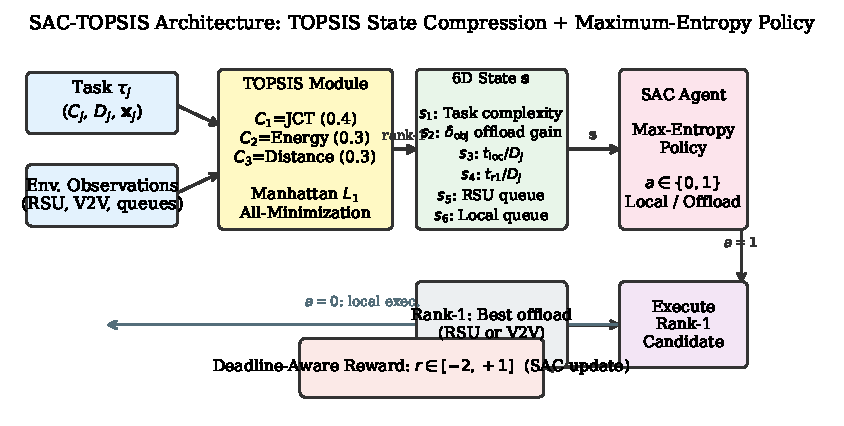
\includegraphics[width=\columnwidth]{images/fig_01_architecture.pdf}
  \caption{\acrotip{SAC}-\acrotip{TOPSIS} Architecture.
           \acrotip{TOPSIS} compresses the variable-sized set of candidates into a
           fixed 6D scale-invariant state vector.
           \acrotip{SAC} learns a binary policy (local vs.\ best offloading)
           over this representation using maximum entropy regularization.}
  \label{fig:architecture}
\end{figure}

\subsection{\acrotip{TOPSIS}-Based State Compression}
\label{sec:topsis}

\paragraph{Decision matrix.}
For task $\tau_j$, we construct a decision matrix
$\mathbf{X} \in \mathbb{R}_{\ge 0}^{3\times 3}$ whose rows correspond to the
three candidate modes (local, \acrotip{RSU}, \acrotip{V2V}) and whose columns are the three
cost criteria:
\begin{equation}
  \mathbf{X} =
  \begin{bmatrix}
    \mathrm{JCT}_j^{(0)} & E_j^{(0)} & 0 \\
    \mathrm{JCT}_j^{(1)} & E_j^{(1)} & d_{\mathrm{RSU}} \\
    \mathrm{JCT}_j^{(2)} & E_j^{(2)} & d_{\mathrm{V2V}}
  \end{bmatrix},
  \label{eq:dm}
\end{equation}
where $d_{\mathrm{RSU}}$ and $d_{\mathrm{V2V}}$ are the Euclidean distances
to the \acrotip{RSU} and the selected \acrotip{V2V} pair, respectively.
If a mode is unfeasible, its row is set to $10^6$ to exclude it from the
ideal solutions.

\paragraph{Weighted normalization.} Each column $j$ is normalized by its Euclidean norm $\|\mathbf{X}_{:j}\|_2$ and then multiplied by the weight $w_j \in \{0.4;\, 0.3;\, 0.3\}$ (\acrotip{JCT}, energy, distance), resulting in the weighted normalized matrix $\widetilde{\mathbf{X}}$.

\paragraph{\acrotip{TOPSIS} $L_1$-Manhattan.}
We differ from classic \acrotip{TOPSIS} by measuring distances to the positive ideal solution (\acrotip{PIS})
$A^+$ and the negative ideal solution (\acrotip{NIS}) $A^-$ using the Manhattan norm
($L_1$):
\begin{equation}
  D_i^+ = \textstyle\sum_{k} \lvert \widetilde{x}_{ik} - A_k^+ \rvert,
  \qquad
  D_i^- = \textstyle\sum_{k} \lvert \widetilde{x}_{ik} - A_k^- \rvert.
  \label{eq:manhattan}
\end{equation}
The closeness score is then $\mathcal{C}_i = D_i^- / (D_i^+ + D_i^-)$.
Since all criteria are cost minimization objectives, $A^+$ is the
column-wise minimum and $A^-$ is the column-wise maximum of
$\widetilde{\mathbf{X}}$.
The $L_1$ metric is less sensitive to extreme values, a critical property when
queue estimates are noisy, and is computationally lighter than $L_2$.

\paragraph{Rank-1 selection.}
The rank-1 offloading candidate is the feasible non-local mode with the
highest $\mathcal{C}_i$:
\begin{equation}
  m^* = \operatorname*{argmax}_{i \in \{1,2\}} \mathcal{C}_i
        \;\text{s.t.\ mode } i \text{ is feasible}.
  \label{eq:rank1}
\end{equation}
Ties are resolved in favor of \acrotip{V2V} to encourage load balancing.
If no offloading mode is feasible, $m^*$ reverts to local execution
regardless of the agent's action.

\paragraph{6D state vector.}
The state $\mathbf{s} \in \mathbb{R}^6$ is assembled as:
\begin{align}
  s_1 &= C_j / 10^{10} \notag \\
  s_2 &= \mathrm{clip}\!\left(1 - \frac{\mathrm{cost}_{m^*}}{\mathrm{cost}_{\mathrm{loc}}},\,-1,1\right) \notag \\
  s_3 &= \min\!\left(1,\; \mathrm{\acrotip{JCT}}^{(0)} / D_j\right) \notag \\
  s_4 &= \min\!\left(1,\; \mathrm{\acrotip{JCT}}^{(m^*)} / D_j\right) \notag \\
  s_5 &= \min\!\left(1,\; |Q_{\mathrm{\acrotip{RSU}}}| / 25\right) \notag \\
  s_6 &= \min\!\left(1,\; |Q_{v_0}| / 25\right)
  \label{eq:state}
\end{align}
{\scriptsize where the components represent: task complexity; offloading advantage; local urgency; rank-1 urgency; \acrotip{RSU} queue occupancy; and local queue occupancy.}
where $\mathrm{cost}_m = \alpha\,\mathrm{JCT}^{(m)} + \beta\,E^{(m)}$.
All components belong to $[0,1]$ or $[-1,1]$, making $\mathbf{s}$
scale-invariant, as it does not depend on the number of available candidates,
only on the relative quality of the best one.

\subsection{Maximum Entropy Soft Actor-Critic}
\label{sec:sac}

The \acrotip{SAC} agent optimizes the maximum entropy objective~\cite{haarnoja2018sac}:
\begin{equation}
  \pi^* = \operatorname*{argmax}_\pi\;
  \mathbb{E}_{\tau \sim \pi}\!\left[
    \sum_{t} \gamma^t \bigl(r_t + \alpha_T\,\mathcal{H}[\pi(\cdot\mid s_t)]\bigr)
  \right],
  \label{eq:sac_obj}
\end{equation}
where $\alpha_T$ is the automatically adjusted temperature parameter.
The actor and critic networks are MLPs with two hidden layers of 256 units and
ReLU activations.
The actor generates logits for the Bernoulli action distribution; the temperature
$\alpha_T$ is adapted to a target entropy of $\log 2 / 2$ nats.
The replay buffer stores $10^5$ transitions; the mini-batch size is $256$;
the learning rate is $3 \times 10^{-4}$ for all networks.

\paragraph{Why binary action?} Delegating the selection of the offloading destination to \acrotip{TOPSIS} reduces the action space from $|\mathcal{V}(t)| + 2$ dimensions to a single bit. This simplification is lossless from the agent's perspective, as the relative ordering of candidates is already encoded in $s_2$--$s_4$.

\subsection{Deadline-Aware Reward Function}
\label{sec:reward}

The reward $r_j$ for task $\tau_j$ is designed to guide the agent toward
deadline fulfillment while providing a continuous gradient signal:
\begin{equation}
  r_j = \begin{cases}
    1.0 - 0.5 \cdot \rho_j        & \text{if } \mathrm{JCT}_j \le D_j, \\
    -1.0 - \min(1,\,\delta_j)       & \text{otherwise,}
  \end{cases}
  \label{eq:reward}
\end{equation}
where
\begin{equation}
  \rho_j = \tfrac{1}{2}\!\left(\frac{\mathrm{JCT}_j}{D_j}
                              + \frac{E_j}{E_{\max,j}}\right) \in [0,1]
  \label{eq:rho}
\end{equation}
is a normalized cost ratio, and $\delta_j = (\mathrm{JCT}_j - D_j)/D_j$
is the relative deadline violation.
Successful executions yield $r_j \in [0.5,\,1.0]$: faster and more
efficient tasks receive higher rewards.
Failed executions yield $r_j \in [-2,\,-1]$: the penalty grows with the
degree of delay, providing a gradient that teaches the agent to
fail for the shortest possible time.
